%!TEX root = ../BoYu-Dissertation.tex
\graphicspath{{Figures/}}
\chapter{Understanding Awareness} % (fold)
\label{cha:understanding_awareness}
This chapter attempts to identify the major issues for understanding awareness phenomena in complex, distributed collaborative activities. A review of what is currently known about awareness phenomena in collaboration is presented, which provides the ground work for our conceptual model in next chapter.

Following the discussion in \cite{Gutwin2002}, we organize the discussion of awareness phenomena around three issues:

\begin{enumerate}
   \item What kinds of awareness information are needed for human activities? (Section \ref{sec:concepts_of_awareness})
   \item How do people maintain and develop awareness in the process of activities? (Section \ref{sec:development_of_awareness})
   \item How do people share and distribute awareness knowledge in collaboration? (Section \ref{sec:awareness_in_collaboration})
\end{enumerate}

Findings in these three areas inform three design-related research questions to support awareness: what information to gather and distribute, how to present the information to the user, and how to support the team to share awareness knowledge. The remainder of this chapter is organized around these three issues respectively. First, we review the existing awareness concepts on what the awareness knowledge is composed of. Then we discuss existing cognitive models on awareness process. Last we discuss how shared and distributed awareness is achieved in collaborative settings.

\section{Concepts of awareness} % (fold)
\label{sec:concepts_of_awareness}
The concept of awareness has come to play a central role in CSCW research. However, what in CSCW labeled as `awareness' has little in common, besides the fact that it represents some aspect of human interaction that is important for successful collaboration \cite{schmidt2002a}. In this section, we identify three related types of awareness in the literature that reflect the evolving understanding of the awareness phenomena (Figure \ref{fig:concepts_of_awareness}): (1) \emph{situation awareness} that emphasizes individual actor's knowledge about the working environment, (2) \emph{team awareness} including the awareness knowledge about other team members and their activities, (3) and \emph{activity awareness} that entails both situation awareness and team awareness, and emphasizes the collective knowledge of the shared collaborative activity as a whole.

\begin{figure}[htbp] %  figure placement: here, top, bottom, or page
   \centering
   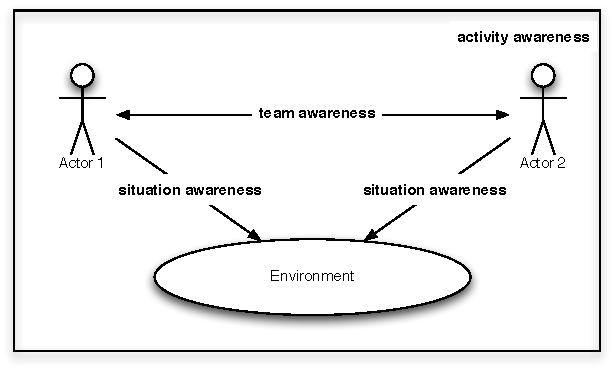
\includegraphics{concepts_of_awareness.pdf} 
   \caption{Concepts of awareness}
   \label{fig:concepts_of_awareness}
\end{figure}


\subsection{Situation awareness} % (fold)
\label{sub:situation_awareness}
Research into awareness originated from the study of situation awareness (SA) in the human factors research community. Situation awareness is considered as knowledge created through interaction between a person and his/her environment, i.e. ``knowing what is going on'' in the situation \cite{Endsley1995}. Situation awareness emphasizes the knowledge about the environment that an actor's activities are situated in, i.e. awareness is knowledge about the state of an environment bounded in time and space \cite{Adams1995}.

Although most of existing situation awareness models in the literature are individual focused theories \cite{Salmon2008}, it has also been well recognized as an important element in collaborative environments. Gutwin and Greeenberg \cite{Gutwin2002} view their workspace awareness as a specialization of situation awareness tied to the specific setting of the shared workspace. The concept of activity awareness proposed by Carroll et al. \cite{carroll2003a} also subsumes situation awareness with an emphasis on aspects of the situation that have consequences for group work towards shared goals. In the context of collaborative activities, situation awareness emphasizes the awareness of the object of collaboration, e.g. the environment in which the collaboration occurs.
% subsection situation_awareness (end)
\subsection{Team awareness} % (fold)
\label{sub:team_awareness}
Awareness in collaborative environments is indubitably more complex than awareness at the individual level. Beyond knowing what is going on in the environment, i.e. situation awareness, team members also need to develop an understanding of each other and their actions to ensure that individual contributions are relevant to the group's shared goal as a whole \cite{dourish1992awareness}. 

In a broad sense, two types of awareness can be distinguished in CSCW research: \emph{social} awareness and \emph{task-oriented} awareness \cite{prinz1999a,schmidt2002a,carroll2003a}.

\emph{Social} awareness addresses the availability of different kinds of information related to the social context of team members, e.g. awareness about what they are doing, if they are talking to someone, if they can be disturbed etc. \emph{Social} awareness thus is conceived of as something that engenders ``informal serendipitous interactions'' \cite{hudson1996a} and ``a shared space for community building'' \cite{Dourish1992}. Awareness of the general social context is an important aspect of collaborative work, especially in domains where cooperative work is defined in a loose and broad sense, or domains where socialization is crucial \cite{schmidt2002a}.

However, when the tasks of collaborators become closely interdependent, more urgent concerns need to be given to the aspect of \emph{task-oriented} awareness. The \emph{task-oriented} awareness focuses on practices through which actors seamlessly align and integrate their distributed, yet interdependent actions. During these practices, people become aware of what tasks have been done or what are in need of being done. They understand how other team members' actions can be advantageous or detrimental for their own work, and make necessary adjustments to intended course of actions \cite{schmidt2002a}. The major difference of \emph{task-oriented} awareness from \emph{social} awareness is that it focuses on tasks performed to achieve a specific shared goal \cite{carroll2003a} and the actor's being interdependent in their work \cite{schmidt2002a}.
% subsection team_awareness (end)

\subsection{Activity awareness} % (fold)
\label{sub:activity_awareness}
In collaborative activities, situation and team awareness are equally important. On one hand, because of the distributed nature of collaborative activities, the situation awareness is associated with individual actors, as each actor must be able to perceive the elements in the environment related to their own actions. On the other hand, to ensure that different actors' actions are aligned with each other, the actors have to develop team awareness of each other. For instance, in the context of geo-collaboration, MacEachren and Brewer \cite{Maceachren2004} studied the important roles of maps as an awareness artifact in collaboration. On one hand, maps provide the situation awareness by providing the geo-context of the collaborative environments. Meanwhile, they are used to compare perspectives, mediate among knowledge domains of participants, and enable joint activity .

To provide a more comprehensive understanding of awareness in collaborative environment, Carroll et al. proposed the concept of `activity awareness' \cite{carroll2003a,carroll2006a}. In framing activity awareness, they appropriated the concept of \emph{activity} from Activity Theory to provides a level of abstraction that can cover both situation awareness and team awareness, and emphasize that collaborators need to be aware of a shared activity as a complex, socially embedded endeavor, organized in dynamic hierarchies. 

Comparing with situation awareness and team awareness, we believe that the concept of activity awareness provides a more adequate framework to structure the major elements of awareness knowledge in complex, distributed collaboration. 
\begin{enumerate}
   \item Situation awareness focuses on the awareness of objects and artifacts in the environment where collaborative activities are embedded. This is adequate when the tasks of team members are loosely coupled and clearly defined, so that each of them can merely focuses on the part of the environment that is relevant to his/her task. However, in complex collaboration as we discuss here, tasks of different actors are closely interdependent. To work together as a team, people cannot just work inside his/her local environment, but also need adequate awareness knowledge from each other.
   \item On the other hand, team awareness emphasizes how team members develop and share awareness knowledge of each other. However, what is missing in team awareness is how knowledge about objects and events in the external environment can interact with the awareness knowledge about other team members. An event in my local environment may not be relevant to my own work, but rather is related to another team member's task. By knowing the other team member's work, I can pass the event to him/her so that he/she can develop a better situation awareness. In this way, the situation awareness and team awareness are meshed up together to form the collective awareness at the team level. 
   \item Built on top of situation awareness and team awareness, activity awareness emphasizes the importance of using the concept of activity to structure the awareness phenomena at the collective level. The ultimate motivation of human actors to acquire and maintain awareness in a collaborative environment is to achieve their shared goals by performing their activities. As a result, no matter whether the knowledge comes from the external environment (i.e. situation awareness), or internal tasks and status (i.e. team awareness), as long as it is needed for the team to achieve their shared goals, it becomes relevant awareness information. By modeling and analyzing the activity structure behind the awareness phenomena, we can understand the requirements for awareness knowledge in complex and dynamic collaborations from a more systematical perspective.
\end{enumerate}

% subsection activity_awareness (end)
% section concepts_of_awareness (end)
\section{Development of awareness} % (fold)
\label{sec:development_of_awareness}
In the literature, it has been well recognized that the achievement of awareness is much more than just providing the human actors with enough awareness information. Rather, it should be considered as a complex process through which awareness is obtained and developed. 

Among the numerous attempts to specify the development of situation awareness \cite{Salmon2008}, Endsley's three-level model \cite{Endsley1995} has undoubtedly received the most attention. The three-level model describes situation awareness as a cognitive process comprising three steps and during each step, the level of awareness is increased \cite{Endsley1995}:

\begin{enumerate}
   \item Level 1: \emph{perception of relevant elements in the environment}. An actor must first be able to gather perceptual information in the surrounding environment, and be able to selectively attend to those elements that are most relevant for the task at hand. At this stage, the information is merely perceived and no further processing takes place. 
   \item Level 2: \emph{Comprehension of task-related elements in Level 1}. Level 2 involves the interpretation of the perceptual information from Level 1 in a way that allows an actor to comprehend or understand its relevance in relation to their tasks and goals.
   \item Level 3: \emph{Projection of the states in the near future}. Using a combination of Level 1 and Level 2 awareness-related knowledge and experience in the form of mental models, an actor can forecast likely future states in the situation.
\end{enumerate}

Endsley's three-level model presents an intuitive description of how situation awareness is developed at the individual level and has been applied in a plethora of different domains \cite{Wickens2008}. The division of SA into three levels allows the construct to be measured easily and effectively \cite{endsley1995measurement}, and also supports the abstraction of awareness requirements and the development of design guidelines \cite{Salmon2008}. Furthermore, it has been extended in order to describe team situation awareness \cite{endsley2001model}, and the three levels of awareness information are applicable in many collaborative situations \cite{Gutwin2002}.

However, an important flaw of the three-level mode is its focus on the internal cognitive process of human actors, without considering changes in the external environment. This leads to the inability to cope with the activities that are situated in the environment that changes over time \cite{Smith1995,uhlarik2002review}. To investigate the effect of situational changes to awareness, many researchers have used Niesser's perceptual cycle model \cite{neisser1976cognition} to clarify the cognitive components involved in the acquisition and development of situation awareness \cite{Smith1995,Adams1995,Gutwin2002,Stanton2009}. According to the perceptual cycle model (Figure. \ref{fig:perceptual_cycle}), an actor's interaction with the world continues in an infinite cyclical nature. By perceiving the available information in the environment, the actor modifies its knowledge. Knowledge directs the actor's activity in the environment. That activity samples and perhaps anticipates or alters the environment, which in turn informs the actor. The informed, directed sampling and/or anticipation capture the essence of behavioral characteristic of situation awareness.

\begin{figure}[htbp] %  figure placement: here, top, bottom, or page
   \centering
   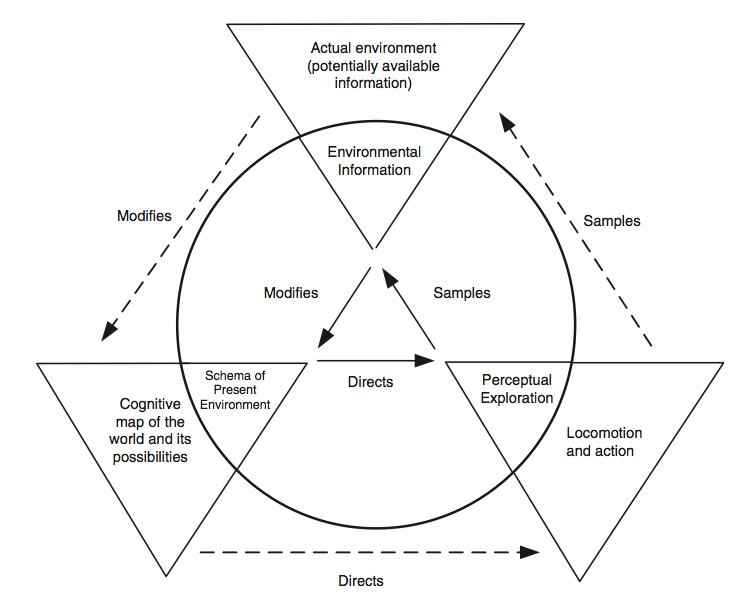
\includegraphics[width=4.5in]{perceptual_cycle.jpg} 
   \caption{Niesser's perceptual cycle model \cite{Salmon2008}}
   \label{fig:perceptual_cycle}
\end{figure}

Based upon Niesser's perceptual cycle model, Smith and Hancock suggest that situation awareness is neither resident in the world nor in the person, but resides through the interaction of the person with the world \cite{Smith1995}. Thus they view situation awareness as a generative process in ``an adaptive cycle of knowledge, action and information'' \cite{Smith1995}. In a similar fashion, Adams et al. \cite{Adams1995} used a modified version of Niesser's perceptual cycle model to describe how situation awareness works. They argue that the process of achieving and maintaining situation awareness revolves around an internally held mental model, which facilitates the anticipation of situational events, draw an actor's attention to cues in the environment and directs their eventual course of action. An actor then conducts checks to confirm that the evolving situation conforms to expectations. Any unexpected events serve to prompt further search and explanation, which in turn modifies the actor's existing model. Gutwin and Greeenberg \cite{Gutwin2002} used the perception-action cycle to explain how the awareness is maintained in a shared workspace, in which awareness knowledge both directs and is updated by perceptual exploration of the workspace environment.

One of the key assumptions of these models is the interplay between the awareness information and the internal mental model of current situation. In the process of awareness development, some knowledge is activated and integrated into the mental model, while some becomes inactive or removed from the mental model. Although Smith and Hancock suggested that the adaptation of awareness information into the mental model should be goal-directed, i.e. it must reside in the task environment rather than in the actor's head \cite{Smith1995}, little detail has been given about the cognitive processes that guide the selection and interpretation of awareness information into the mental models.

In an attempt to clarify the cognitive processes involved in the development of awareness, Bedny and Meister \cite{Bedny1999} proposed a description of situation awareness based on the activity theory. They purport that individuals possess goals that represent an ideal image or desired end states of activities, which direct their actions to achieve these goals. It is the difference between the goals and the current situation that motivates an individual to engage in the awareness process and take action towards achieving the goal. Based on the activity theory, Bedny and Meister emphasize how the actor's goals and actions play a central role in the process of awareness development. Critical environmental features are identified based upon their significance to the individual's actions and the individual's motivation towards the task goal. The interpretation of these features in turn modifies an individual's goals and conceptual model of the current situation, which directs their activities and interaction with the world.
% section development_of_awareness (end)

\section{Collaborative awareness} % (fold)
\label{sec:awareness_in_collaboration}
Although awareness in collaboration entails the situation awareness and team awareness at the individual level, there is a lot more to awareness at the team level than merely combining each team's individual awareness \cite{salas1995situation}. To ensure that different actor's individual awareness is compatible with each other, and together results in a coordinated and complete team-level awareness of the collaborative activity, the actors have to interact with each other through team processes.

This section reviews three prominent conceptualizations of collaborative awareness: team situation awareness, activity awareness, and distributed team awareness. These studies aim to explain how the team-level awareness is borne out of the interactions among individual actors, from both the `product' and the `process' aspects (Table \ref{tab:collaborative_awareness}). From the `product' aspect, it is to understand the configuration of awareness knowledge in collaborative environments, i.e. how it is composed of the awareness knowledge of individual team members. From the `process' aspect, it is to understand the interaction between team members through which the collaborative awareness is developed. 
\begin{table}[htbp]
\centering
\footnotesize
\begin{tabular}{>{\raggedright}p{1.1in}>{\raggedright}p{2.2in}>{\raggedright}p{2.2in}}
   \toprule 
    & \textbf{The `product' of awareness} & \textbf{The `process' of awareness}\tabularnewline
   \midrule 
   Collaborative awareness as shared knowledge & individual team member\textquoteright{}s awareness and the shared
   awareness knowledge with other team members & effective team processes for sharing relevant information, such as
   communication and mutual monitoring\tabularnewline
   \midrule 
   Collaborative awareness as shared activities & the shared context surrounding a collaborative activity, e.g. the shared
   goals and status, the top-down goal decomposition, the dependencies
   within the actions, etc. & the joint construction of common ground, shared practices, social
   capital, and human development\tabularnewline
   \midrule 
   Collaborative awareness as distributed cognition & distributed individual awareness that is overlapping, and complementary
   with each other & transactions representing the exchanging of awareness between actors\tabularnewline
   \bottomrule
\end{tabular}  
\caption{Conceptualizations of collaborative awareness}
\label{tab:collaborative_awareness}
\end{table}

\subsection{Collaborative awareness as shared knowledge} % (fold)
\label{sub:team_situation_awareness}
The research on team situation awareness (TSA) attempts to directly extend the theories and models of situation awareness to collaborative settings. TSA conceives the collaborative awareness as a `shared understanding' of the same situation. Endsley et al. \cite{endsley2001model} suggest that, during team activities, situation awareness can overlap between team members, in that individuals need to perceive, comprehend and project awareness elements that are specifically related to their roles in the team, but also elements that are shared with other members in the team. It is therefore argued that, at a simple level, the collaborative awareness comprises two separate but related components: team member's individual awareness, and the shared awareness with other team members (Figure \ref{fig:tsa}). 

\begin{figure}[htbp] %  figure placement: here, top, bottom, or page
   \centering
   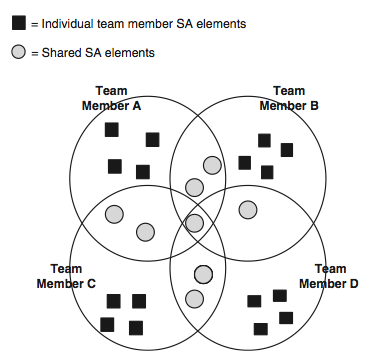
\includegraphics[width=3.5in]{TSA.jpg} 
   \caption{Shared situation awareness (adapted from Endsley 1995 \cite{Endsley1995})}
   \label{fig:tsa}
\end{figure}

The team situation awareness adopts the knowledge-in-common view \cite{Mohammed2001}, i.e. it focuses on how the shared understanding of the situation is developed at the team level. Nofi \cite{nofi2000defining}, for example, defines team SA as: ``a shared awareness of a particular situation'' and Perla et al. \cite{perla2000gaming} suggest that ``shared SA implies that we all understand a given situation in the same way''. Shu and Furuta \cite{shu2005inference} point out that TSA comprises both individual SA and mutual awareness and can be defined as ``two or more individuals share the common environment, up-to-moment understanding of situation of the environment, and another person's interaction with the cooperative task''. As a result, a critical factor of team situation awareness is to define the configuration of shared awareness requirements, i.e. to identify the awareness knowledge that needs to be shared with the team.

By considering the collaborative awareness as shared knowledge among team members, the development of awareness at the team level relies on effective team processes for sharing relevant information. Salas et al. \cite{salas1995situation} propose a framework of TSA that comprises two critical processes, individual situation awareness and team processes. The development of collaborative awareness has a cyclical nature of developing individual SA, sharing SA with other team members, and then modifying SA based on other team members' SA. Most researchers have focused on communication as the key team process in the development of collaborative awareness. Nofi \cite{nofi2000defining}, for example, cites communication as the most critical element in the creation of shared SA . Salas et al. \cite{salas1995situation} argue that team members acquire individual awareness, and then communicate this throughout the team, which leads to a common team understanding. Entin and Entin \cite{entin2000assessing} note that communication is a prerequisite for high levels of team SA. Another key team process that is critical to team SA is the process of mutual monitoring, whereby team members monitor one another's activities, allowing the sharing of awareness information without explicit verbal communication \cite{Gutwin2002,Salmon2008}. Although it is recognized that an increased level of team processes will lead to enhanced levels of team situation awareness. However, the specific relationships between team situation awareness and team processes remains largely unexplained \cite{Salmon2008}.

The heavy emphasis of collaborative awareness on shared knowledge is simplistic in complex, distributed collaboration. As argued by Mohammed and Dumville \cite{Mohammed2001}, the knowledge-in-common view may be appropriate for only certain task domains and types of groups. In teams with high level of division of work, the distribution of knowledge and skills across the team typically is not uniform; as a result, a high level of overlapping knowledge in such teams might be inefficient. As we characterize the collaboration as highly distributed where collaborators play specialized roles or attain distinct knowledge in the course of joint activities, they experience the situation in different ways. So whilst some of the information required by two different team members may be `shared' in the sense that they both need to attend to it as part of their job, their resultant understanding and use of it is different \cite{Salmon2010}.
% subsection team_situation_awareness (end)

\subsection{Collaborative awareness as shared activities} % (fold)
\label{sub:activity_awareness}
To address the problem of the `shared knowledge' view of collaborative awareness, activity awareness \cite{carroll2003a,carroll2006a} emphasizes the importance of using the concept of activity to structure the product and process of awareness phenomena. The ultimate motivation of human actors to acquire and maintain awareness in the collaborative environment is to achieve their shared goals by performing their activities. As a result, the context surrounding a collaborative activity, i.e. the manner in which a shared activity is decomposed into smaller inter-related tasks, how these subtasks are assigned or adopted by collaborators, and when and how distributed subtasks are interdependent on each other, becomes the most important aspects of the situation that the team members need to be aware of \cite{carroll2003a}.

By shifting the focus from shared knowledge to shared activities, activity awareness aligns the development of awareness with the development of collaborative activities. Most basically, activity awareness is achieved and developed through the joint construction of common ground - shared knowledge and beliefs, mutually identified and agreed upon by members through a rich variety of communication protocols \cite{carroll2006a}. In long-term, open-ended activities over significant spans of time, the construction of shared practices, social capital, and human development become also important to develop team member's activity awareness.

Activity awareness with its basis on Activity Theory, provides a level of abstraction that is more constructive and dynamic to structure the sharing requirement in collaborative awareness. The activity awareness focuses on the sharing of activities, i.e. the importance of a common picture of the shared collaborative activities. However, such a common picture is usually distributed in the whole group, instead of in any single actor's mind \cite{Stanton2009}. Each actor in the group has their own awareness, related to the goals they are working towards. However, this seldom includes the whole picture of the collaborative activity, and only when all the actors' awareness knowledge is meshed up together, the common picture emerges. Activity awareness framework provides little detail about how the activity knowledge is distributed across multiple actors.
% subsection activity_awareness (end)

\subsection{Collaborative awareness as distributed cognition} % (fold)
\label{sub:distributed_team_awareness}
A more recent theme to conceptualize awareness in collaboration is the concept of distributed or systemic team awareness \cite{Stanton2009,artman1998situation}. Distributed team awareness approaches are borne out of the distributed cognition theory \cite{hutchins1995cognition}, which describes the notion of joint cognitive systems comprising the people in the system and the artifacts that they use. Within such systems, cognition is achieved through coordination between the system units \cite{artman1998situation} and is therefore viewed as an emergent property (i.e. relationship between systemic elements) of the system rather than an individual endeavor. Distributed team awareness approaches therefore view awareness in collaboration not as a shared understanding of the situation, but rather as a characteristic of the socio-technical system itself \cite{artman1998situation}. Whilst recognizing that team members possess their individual SA for a particular situation and that they may share their understanding of the situation, distributed team awareness assumes that awareness is distributed across different human and technological agents involved in collaborative systems \cite{Stanton2009}.

The main difference between distributed team awareness and other TSA and activity awareness models is related to the concept of \emph{compatible} awareness \cite{Stanton2009}. Distributed team awareness postulates that, within collaborative systems, each team member does not need to know everything, rather they possess the awareness that is needed for their specific tasks. Although different team members may be aware of the same information, this awareness is not shared, since the team members often have different goals and so view the situation differently based on their own tasks and goals. Different team member's individual awareness can be different in content but at the same time is compatible in that it is all collectively needed for the overall team to perform the collaborative activity successfully \cite{Salmon2010}. The team members' individual awareness can be overlapping, and complementary with each other, and hence deficiencies in one actor's individual awareness can be compensated by another actor. To use the analogy of a cog in a machine, each cog does not need to know about all the other cogs, rather it needs only to be able to connect with those cogs adjacent to it (Figure \ref{fig:compatible_awareness}). Thus it is suggested that `compatibility' is the key to collaborative awareness, rather than `sharedness' \cite{Salmon2008a}.

\begin{figure}[htbp] %  figure placement: here, top, bottom, or page
   \centering
   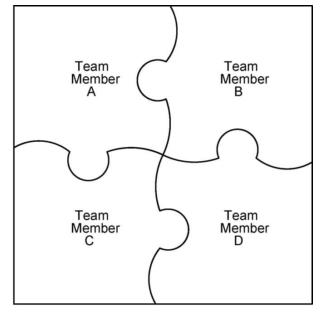
\includegraphics[width=3.1in]{compatible_awareness.jpg} 
   \caption{Compatible awareness (adapted from Salmon et al. \cite{Stanton2009})}
   \label{fig:compatible_awareness}
\end{figure}

While the distributed team awareness emphasizes the distribution of awareness, it does not discount the interactions among different team members. The distributed team awareness is acquired and maintained through \emph{transactions} that arise from communications or other team processes \cite{Salmon2010}. A transaction in this case represents an exchange of awareness knowledge between actors. Actors receive information, integrate it with existing knowledge, and then pass on to other agents. The interpretation on that information changes per team member. Transactions between team members lead to awareness knowledge being passed around. For example, an actor may perceive certain awareness element in the environment, interpret the meaning, and then pass it to another actor via a transaction. The second actor then builds its own interpretation upon the first actor's interpretation, and may start a new transaction to pass his/her understanding to other actors. Hence, it is the systemic transformation of awareness elements as they cross the local boundary from one team member to another that bestows upon awareness in collaboration an emergent behavior \cite{Stanton2009}.

The concept of distributed team awareness has been investigated in a number of domains, including naval warfare \cite{Stanton2006}, energy distribution \cite{Salmon2008a}, and air traffic control \cite{Stanton2009}. The major strength of the approach is related to the systemic approach that it advocates, which is more suitable to analyze the awareness phenomena in complex, real world collaborative activities \cite{Stanton2009}. However, the main weakness, as admitted by the authors, is related to it complexity \cite{Salmon2010}. Similar to other team situation awareness models, it uses concepts as the basic unit to analyze awareness elements, which often leads to extremely large networks in order to represent all the concepts and their relationships in a collaborative environment. A possible remedy is to integrate the distributed team awareness with the activity-directed models (Section \ref{sub:activity_awareness}) and switch the basic unit of analysis from arbitrary concepts to activities to understand the awareness phenomena.
% subsection distributed_team_awareness (end)
% section awareness_in_collaboration (end)

\section{Discussion} % (fold)
\label{cha:understanding_awareness:sec:discussion}
By reviewing the existing theories and conceptual models of awareness, we believe that none of them alone can account for all the aspects of awareness phenomena in complex, distributed collaboration:

\begin{enumerate}
   \item The models of situation awareness primarily focus on the individual level of awareness phenomena, and have limited support for collaborative awareness. 
   \item We agree with the distributed team awareness approaches \cite{Salmon2010} on that, the conceptualization of collaborative awareness merely based on the idea of `sharing' is an oversimplification in complex, distributed collaboration. As we characterize the collaboration as highly distributed where collaborators play specialized roles or attain distinct knowledge in the course of joint activities, the interaction between the actors to achieve collaborative awareness is more about transactions than information sharing.
   \item We resonate with the activity directed SA model \cite{Bedny1999} and the activity awareness framework \cite{carroll2003a} that existing models using concepts as the basic unit to analyze awareness elements tend to be too static and rigid for collaboration with higher level of dynamics.
\end{enumerate}

As a result, instead of adopting one particular viewpoint, we believe that a suitable conceptual model for understanding awareness in complex, distributed collaborative activities should integrate multiple models in the literature. Specifically, we identify the following requirements for such a conceptual model of awareness:

\paragraph*{Integration of individual and collaborative awareness} % (fold)
\label{par:the_integration_of_individual_and_collaborative_awareness}
The conceptual model should be able to account for awareness at both the individual and the team levels, and emphasize how these two aspects interplay with each other. On one hand, because of the distributed nature of these collaborative activities, awareness is associated with individual actors, as each actor must be able to achieve the individual awareness that provides the basis for them to understand each other's work. On the other hand, collaborative awareness requires the actors to interact with each other through team processes so that their individual awareness can be meshed up together.
% paragraph the_integration_of_individual_and_collaborative_awareness (end)

\paragraph*{Support for distributed awareness} % (fold)
\label{par:the_distributed_nature_of_awareness}
Because of the differences in goals, roles, and tasks, each team member's awareness is different in content, but at the same time is compatible for the team to perform the collaborative activity successfully. Hence, the conceptual model should be able to account for how the awareness is distributed across multiple team members, and how they interact with each other to achieve compatibility. 
% paragraph the_distributed_nature_of_awareness (end)

\paragraph*{Integration of awareness model and activity model} % (fold)
\label{par:the_coupling_between_awareness_and_activity}
The conceptual model should emphasizes the importance of using the concept of activity to structure the product and process of awareness phenomena. As pointed out by Schmidt \cite{schmidt2002a}, when we are talking about `awareness', we are talking about the phenomena that actors align and integrate their actions with the actions of others to achieve their shared goals. As a result, any need for the actors to acquire and maintain awareness in the collaborative environment arises out of their need to perform their activities and not for its own sake.
% paragraph the_coupling_between_awareness_and_activity (end)
% section discussion (end)

% chapter understanding_coordination (end)
